\subsection{LQR controller with integral action}
\subsubsection{Introduction TODO}


\begin{figure}[H]
	\centering
	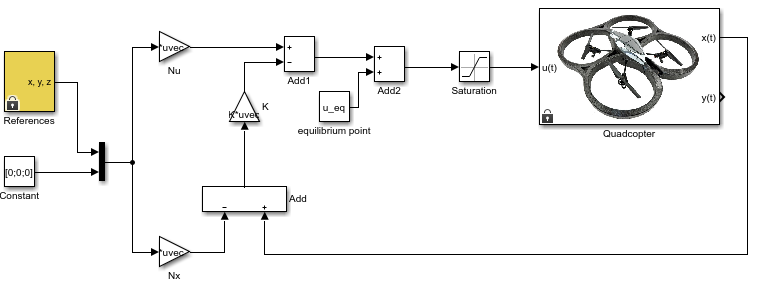
\includegraphics[width=0.5\textwidth]{./LQR_noload/full_state_feedback_simu.png}
	\caption{simulink diagram full-state feedback controller}
	\label{fig:simulink diagram full-state feedback controller}
\end{figure}

\subsubsection{Strategy for finding the weight matrices Q and R}
The x,y, and z are similar to the full state controller, however the integrator can be used to speedup the controller. When increasing the integrator weights weights on the speeds $v_x$,$v_y$ and $v_z$ must be increased to avoid oscillations on the positions x,y and z. Parallel to this R must be properly set to avoid that voltages over 100 can be send to the quad copter as this will obviously not work otherwise.

\subsubsection{Finding the proper weights for the matrix}
The system still contains the elements that simply reduce x,y and z setting these weights to 100 puts the quad copter on the right path. But the performance is very bad, the quad copter flies very slow to its checkpoints. This is displayed in Figure~\ref{fig:step1 integrator}.

\begin{figure}[H]
	\centering
	\begin{subfigure}[b]{0.3\textwidth}
		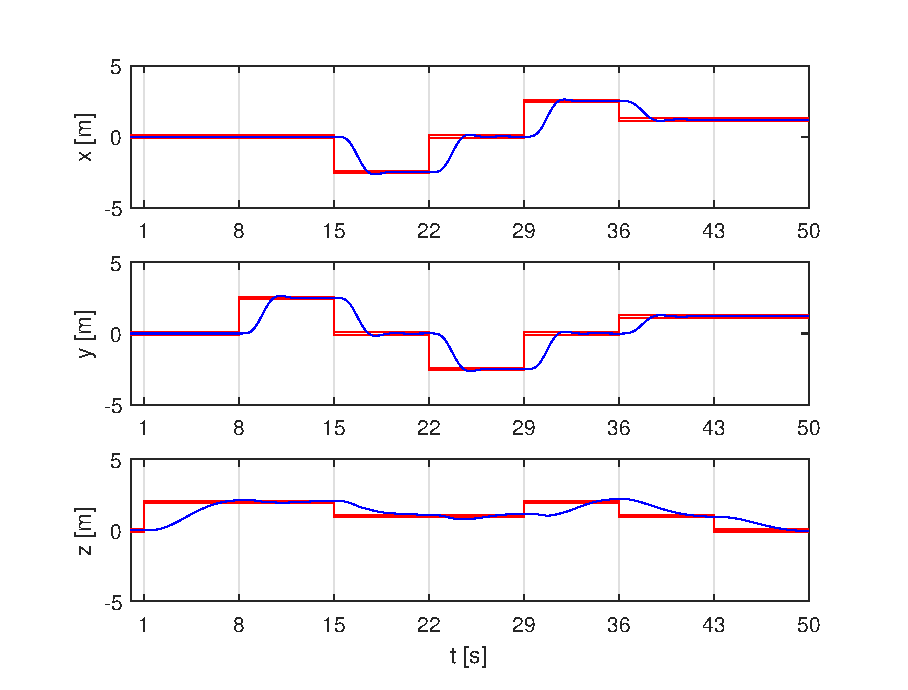
\includegraphics[width=\textwidth]{./LQR_noLoad/integrator/step1_no_integrator_fig3.eps}
		\caption{angles}
	\end{subfigure}
	\begin{subfigure}[b]{0.3\textwidth}
		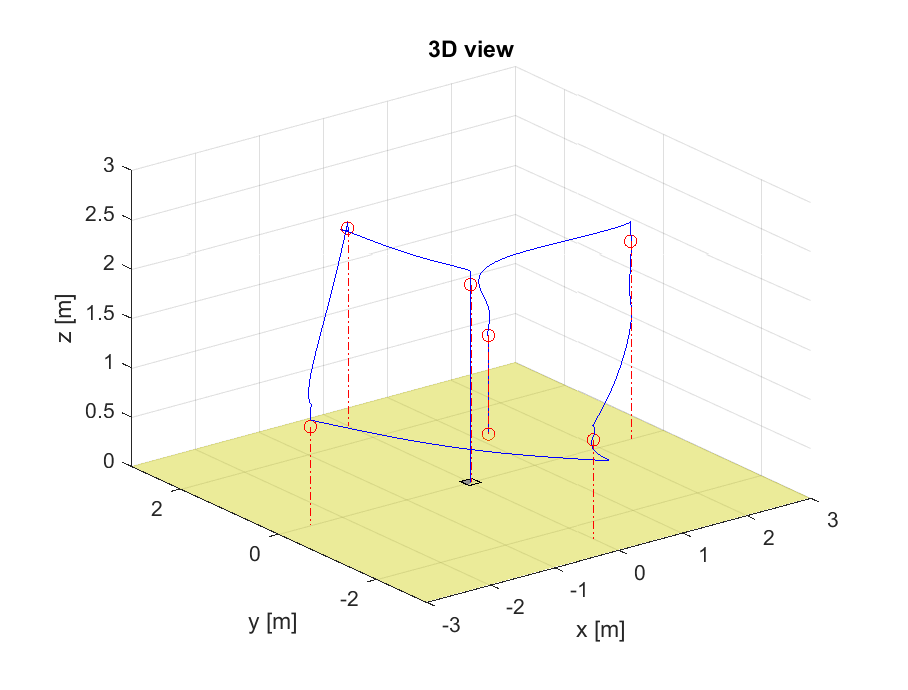
\includegraphics[width=\textwidth]{./LQR_noLoad/integrator/step1_no_integrator_fig2.eps}
		\caption{angles}
	\end{subfigure}
	\caption{step1}\label{fig:step1 integrator}
\end{figure}

A way to speedup the quad copter is to add more weight to the integrators, $10^3$ seems to be an appropriate value. However the quad copter will now "over steer". This will have catastrophic consequences, as the quad copter will  crash! This is displayed in Figure~\ref{fig:step2 integrator} Adding a smaller weight to the integrator will result in oscillations on x,y and z which obviously is not a good thing.

\begin{figure}[H]
	\centering
	\begin{subfigure}[b]{0.3\textwidth}
		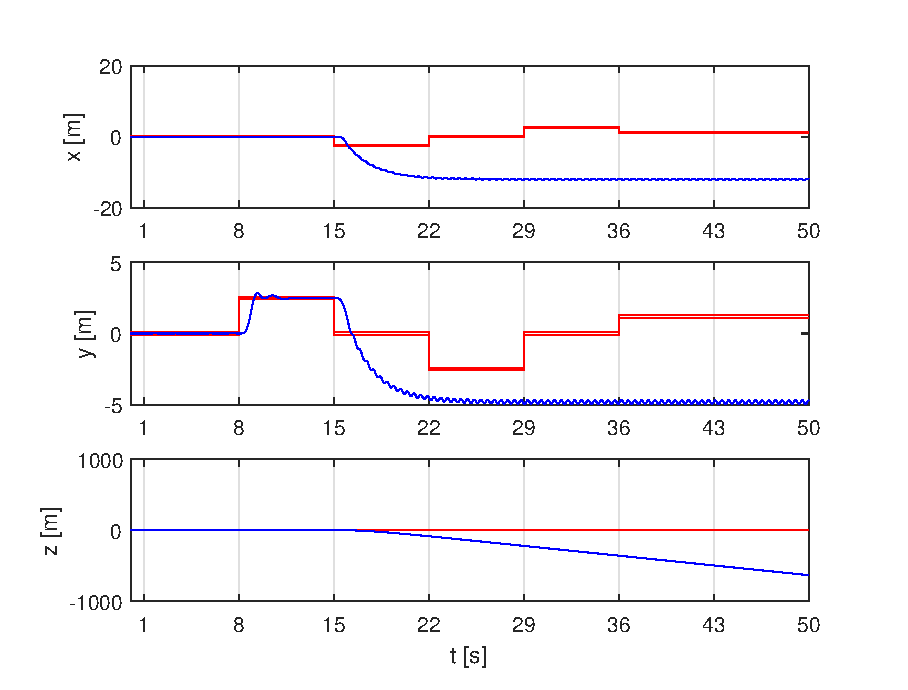
\includegraphics[width=\textwidth]{./LQR_noLoad/integrator/step2_noSpeedLimit_fig3.eps}
		\caption{angles}
	\end{subfigure}
	\begin{subfigure}[b]{0.3\textwidth}
		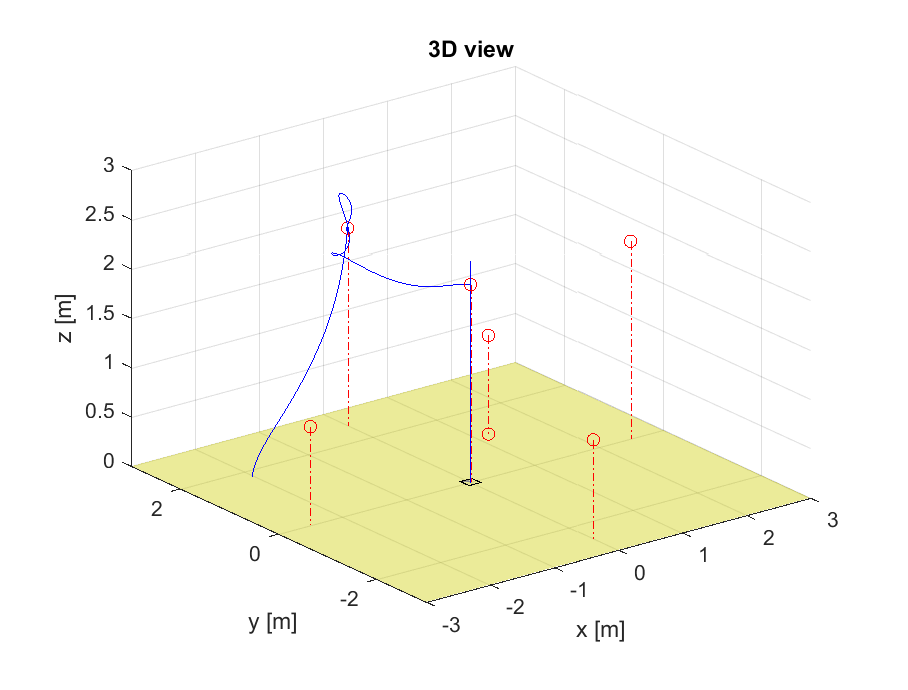
\includegraphics[width=\textwidth]{./LQR_noLoad/integrator/step2_noSpeedLimit_fig2.eps}
		\caption{angles}
	\end{subfigure}
	\caption{step2: adding the integrator}\label{fig:step2 integrator}
\end{figure}

Finally adding a weight to the speed will result in the final result with a total run time of 2.94s. This is displayed in Figure~\ref{fig:step3 integrator}. In addition to these 3 steps the matrix that was set to the value with 50 on its diagonal. This will limit the output so it does not send values over 100 to the quad copter.

\begin{figure}[H]
	\centering
	\begin{subfigure}[b]{0.3\textwidth}
		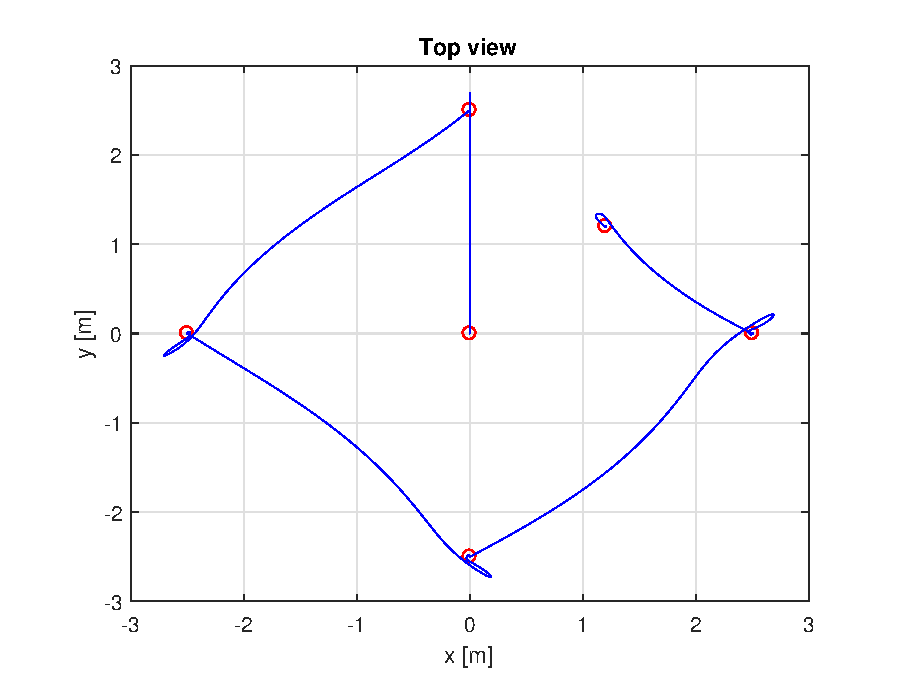
\includegraphics[width=\textwidth]{./LQR_noLoad/integrator/step3_final_fig1.eps}
		\caption{angles}
	\end{subfigure}
	\begin{subfigure}[b]{0.3\textwidth}
		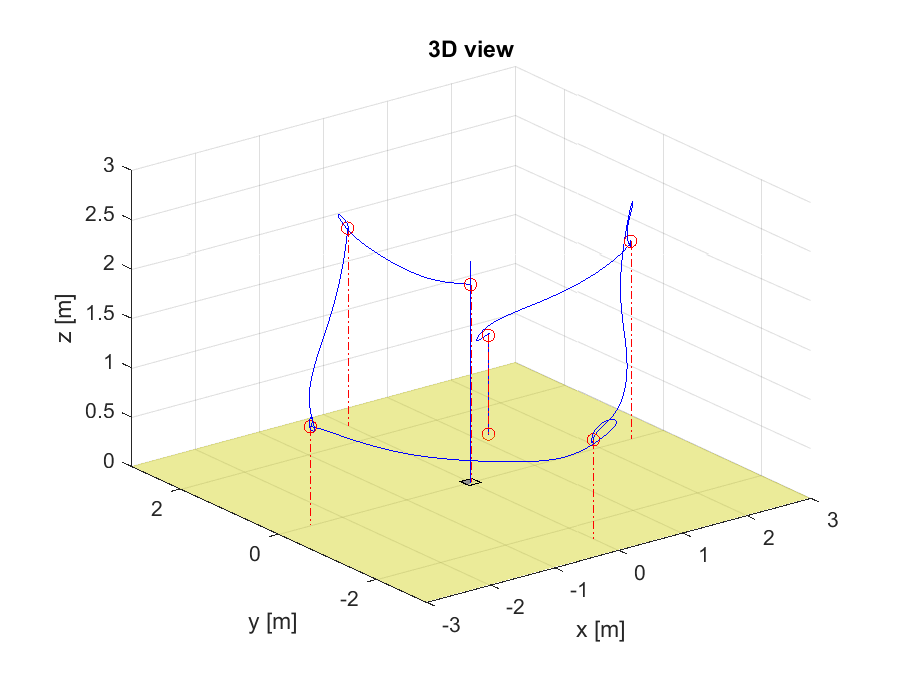
\includegraphics[width=\textwidth]{./LQR_noLoad/integrator/step3_final_fig2.eps}
		\caption{angles}
	\end{subfigure}
	\begin{subfigure}[b]{0.3\textwidth}
		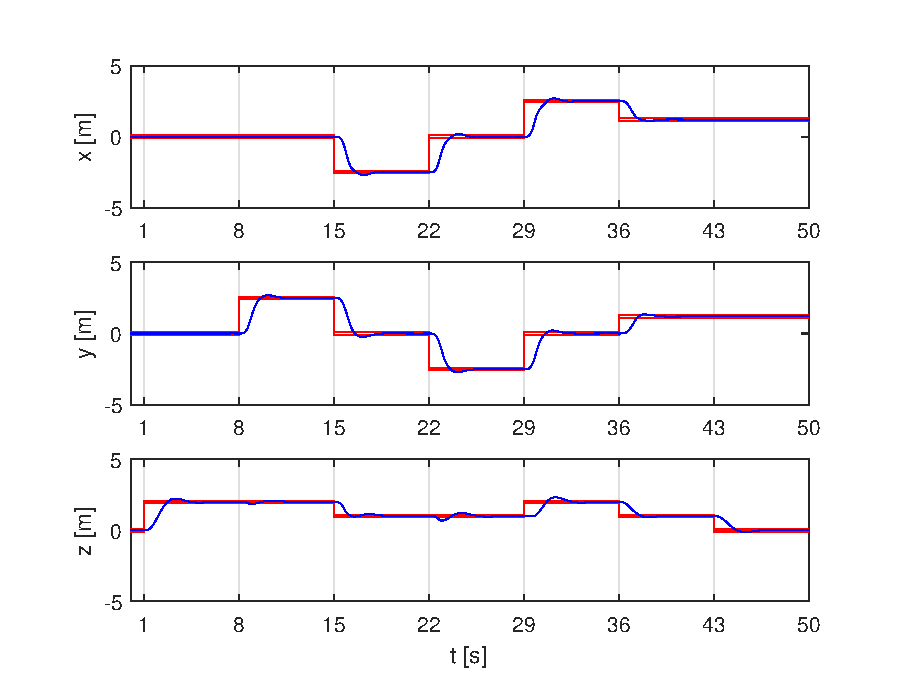
\includegraphics[width=\textwidth]{./LQR_noLoad/integrator/step3_final_fig3.eps}
		\caption{angles}
	\end{subfigure}
	\begin{subfigure}[b]{0.3\textwidth}
		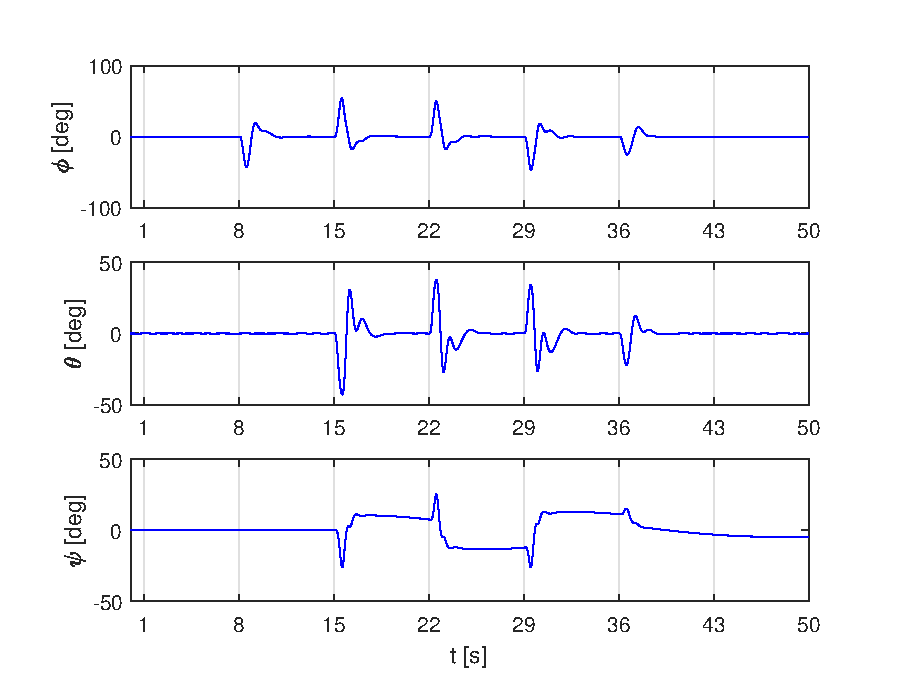
\includegraphics[width=\textwidth]{./LQR_noLoad/integrator/step3_final_fig4.eps}
		\caption{angles}
	\end{subfigure}
	\begin{subfigure}[b]{0.3\textwidth}
		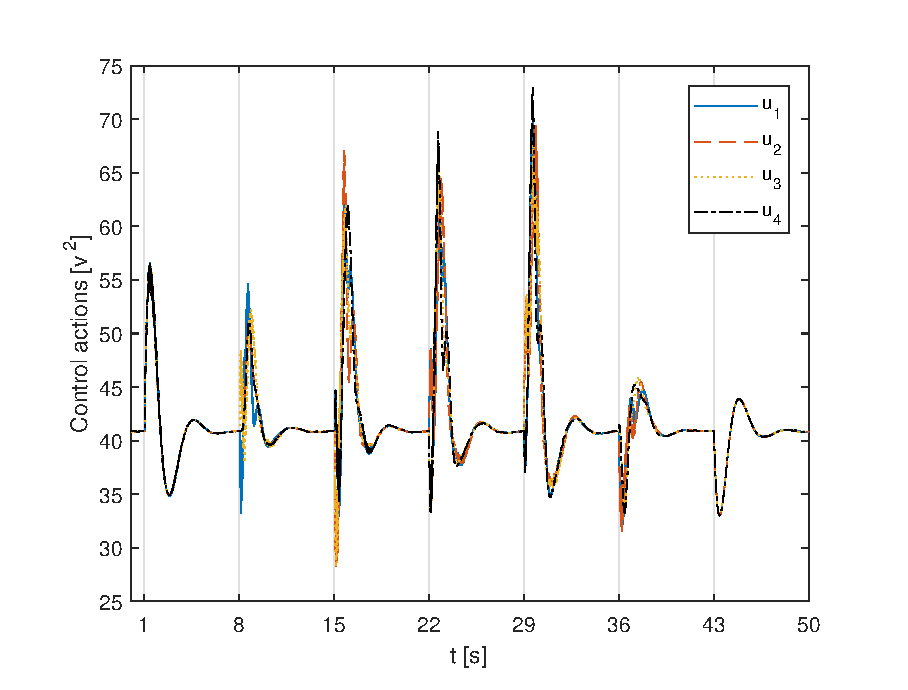
\includegraphics[width=\textwidth]{./LQR_noLoad/integrator/step3_final_fig5.eps}
		\caption{angles}
	\end{subfigure}
	\caption{step3: final results after adding the speed limit}\label{fig:step3 integrator}
\end{figure}

%Timing:
%-------
%From initial pos. to checkpoint 1: 3.050 s
%From checkpoint 1 to checkpoint 2: 2.750 s
%From checkpoint 2 to checkpoint 3: 3.250 s
%From checkpoint 3 to checkpoint 4: 3.200 s
%From checkpoint 4 to checkpoint 5: 3.250 s
%From checkpoint 5 to checkpoint 6: 2.500 s
%From checkpoint 6 to checkpoint 7: 2.750 s

%Average time: 2.964 s
\subsubsection{Final weight matrices}

$$
Q=\begin{bmatrix}
10^3 & 0 & 0 & 0 & 0 & 0 & 0 & 0 & 0 & 0 & 0 & 0 & 0 & 0 & 0 \\
0 & 10^3 & 0 & 0 & 0 & 0 & 0 & 0 & 0 & 0 & 0 & 0 & 0 & 0 & 0 \\
0 & 0 & 10^3 & 0 & 0 & 0 & 0 & 0 & 0 & 0 & 0 & 0 & 0 & 0 & 0 \\
0 & 0 & 0 & 10^2 & 0 & 0 & 0 & 0 & 0 & 0 & 0 & 0 & 0 & 0 & 0 \\
0 & 0 & 0 & 0 & 10^2 & 0 & 0 & 0 & 0 & 0 & 0 & 0 & 0 & 0 & 0 \\
0 & 0 & 0 & 0 & 0 & 10^2 & 0 & 0 & 0 & 0 & 0 & 0 & 0 & 0 & 0 \\
0 & 0 & 0 & 0 & 0 & 0 & 10^4 & 0 & 0 & 0 & 0 & 0 & 0 & 0 & 0 \\
0 & 0 & 0 & 0 & 0 & 0 & 0 & 10^4 & 0 & 0 & 0 & 0 & 0 & 0 & 0 \\
0 & 0 & 0 & 0 & 0 & 0 & 0 & 0 & 1 & 0 & 0 & 0 & 0 & 0 & 0 \\
0 & 0 & 0 & 0 & 0 & 0 & 0 & 0 & 0 & 1 & 0 & 0 & 0 & 0 & 0 \\
0 & 0 & 0 & 0 & 0 & 0 & 0 & 0 & 0 & 0 & 1 & 0 & 0 & 0 & 0 \\
0 & 0 & 0 & 0 & 0 & 0 & 0 & 0 & 0 & 0 & 0 & 1 & 0 & 0 & 0 \\
0 & 0 & 0 & 0 & 0 & 0 & 0 & 0 & 0 & 0 & 0 & 0 & 1 & 0 & 0 \\
0 & 0 & 0 & 0 & 0 & 0 & 0 & 0 & 0 & 0 & 0 & 0 & 0 & 1 & 0 \\
0 & 0 & 0 & 0 & 0 & 0 & 0 & 0 & 0 & 0 & 0 & 0 & 0 & 0 & 1 \\
\end{bmatrix}
$$
$$
R=\begin{bmatrix}
50 & 0 & 0 & 0 \\
0 & 50 & 0 & 0 \\
0 & 0 & 50 & 0 \\
0 & 0 & 0 & 50 \\
\end{bmatrix}
$$